\documentclass[a4paper,11pt]{article}
\usepackage{amsmath,amsthm,amsfonts,amssymb,amscd,amstext,vmargin,graphics,graphicx,tabularx,multicol} 
\usepackage[francais]{babel}
\usepackage[utf8]{inputenc}  
\usepackage[T1]{fontenc} 
\usepackage{pstricks-add,tikz,tkz-tab,variations}
\usepackage[autolanguage,np]{numprint} 

\setmarginsrb{1.5cm}{0.5cm}{1cm}{0.5cm}{0cm}{0cm}{0cm}{0cm} %Gauche, haut, droite, haut
\newcounter{numexo}
\newcommand{\exo}[1]{\stepcounter{numexo}\noindent{\bf Exercice~\thenumexo} : \marginpar{\hfill /#1}}
\reversemarginpar


\newcounter{enumtabi}
\newcounter{enumtaba}
\newcommand{\q}{\stepcounter{enumtabi} \theenumtabi.  }
\newcommand{\qa}{\stepcounter{enumtaba} (\alph{enumtaba}) }
\newcommand{\initq}{\setcounter{enumtabi}{0}}
\newcommand{\initqa}{\setcounter{enumtaba}{0}}

\newcommand{\be}{\begin{enumerate}}
\newcommand{\ee}{\end{enumerate}}
\newcommand{\bi}{\begin{itemize}}
\newcommand{\ei}{\end{itemize}}
\newcommand{\bp}{\begin{pspicture*}}
\newcommand{\ep}{\end{pspicture*}}
\newcommand{\bt}{\begin{tabular}}
\newcommand{\et}{\end{tabular}}
\renewcommand{\tabularxcolumn}[1]{>{\centering}m{#1}} %(colonne m{} centrée, au lieu de p par défault) 
\newcommand{\tnl}{\tabularnewline}

\newcommand{\bmul}[1]{\begin{multicols}{#1}}
\newcommand{\emul}{\end{multicols}}

\newcommand{\trait}{\noindent \rule{\linewidth}{0.2mm}}
\newcommand{\hs}[1]{\hspace{#1}}
\newcommand{\vs}[1]{\vspace{#1}}

\newcommand{\N}{\mathbb{N}}
\newcommand{\Z}{\mathbb{Z}}
\newcommand{\R}{\mathbb{R}}
\newcommand{\C}{\mathbb{C}}
\newcommand{\Dcal}{\mathcal{D}}
\newcommand{\Ccal}{\mathcal{C}}
\newcommand{\mc}{\mathcal}

\newcommand{\vect}[1]{\overrightarrow{#1}}
\newcommand{\ds}{\displaystyle}
\newcommand{\eq}{\quad \Leftrightarrow \quad}
\newcommand{\vecti}{\vec{\imath}}
\newcommand{\vectj}{\vec{\jmath}}
\newcommand{\Oij}{(O;\vec{\imath}, \vec{\jmath})}
\newcommand{\OIJ}{(O;I,J)}


\newcommand{\reponse}[1][1]{%
\multido{}{#1}{\makebox[\linewidth]{\rule[0pt]{0pt}{20pt}\dotfill}
}}

\newcommand{\titre}[5] 
% #1: titre #2: haut gauche #3: bas gauche #4: haut droite #5: bas droite
{
\noindent #2 \hfill #4 \\
#3 \hfill #5

\vspace{-1.6cm}

\begin{center}\rule{6cm}{0.5mm}\end{center}
\vspace{0.2cm}
\begin{center}{\large{\textbf{#1}}}\end{center}
\begin{center}\rule{6cm}{0.5mm}\end{center}
}



\begin{document}
\pagestyle{empty}
\titre{Contrôle 4 : Multiplications et angles }{Nom :}{Prénom :}{Classe}{Date}

\vspace*{0.5cm}

\begin{tabular}{|m{11cm}|c|c|c|}
\hline 
\textbf{Compétences} & \textbf{Acquis} & \textbf{En cours}  & \textbf{Non acquis} \\ 
\hline 
-  Savoir poser et effectuer le produit de nombres décimaux. &  &  & \\
\hline
- Savoir multiplier par 10, 100, 1000 etc... &  &  &  \\ 
\hline 
- Savoir multiplier par 0,1; 0,01 ; 0,001 etc... &  &  &  \\ 
\hline 
- Savoir calculer en ligne de manière astucieuse le produit de plusieurs facteurs. &  &  &  \\ 
\hline 
- Comprendre et s'engager dans la résolution d'un problème.  &  &  &  \\ 
\hline 
- Savoir construire un angle de mesure donnée.  &  &  &  \\ 
\hline 

\end{tabular} 

\vspace*{0.5cm}

Les exercices avec le signe 
\includegraphics[scale=0.4]{trefle.eps}  sont à faire directement sur le sujet. Les autres se font sur la copie double.\\

\vspace*{0.5cm}

\exo{3} Poser et effectuer les opérations suivantes :               

\bmul{3}

284  $\times$ 79\\



\columnbreak

$3,8 \times 7,6$\\

\columnbreak


87 000 $\times$ 0,024\\


\emul

\vspace*{0.5cm}

\exo{4.5} 
\includegraphics[scale=0.4]{trefle.eps}  Compléter par le nombre manquant :\\

\bmul{3}

$3,5 \times 100 =$ . . . \\

$1,7 \times . . . =$ 0,17 \\

$. . . \times 0,1 =$ 1,36 \\


\columnbreak

$1,23 \times 1000 =$ . . . \\

$0,16 \times . . . =$ 1600 \\

$. . . \times 100 =$ 52,5\\

\columnbreak

$17,9\times 0,01 =$ . . . \\

$543  \times . . . =$ 0,543 \\

$. . . \times 1 =$ 27,3 \\

\emul

\exo{3} Calculer astucieusement en détaillant les étapes de calculs.\\

\bmul{2}

$K = 50 \times 12,39 \times 2$\\

\columnbreak

$K = 2,5 \times 7,8 \times 4$\\

\emul



\exo{4}\\
Une famille composée des deux parents, du fils aîné Pierre, âgé de 16 ans, des deux jumelles Mathilde et Noémie, âgées de 8 ans et du petit dernier Gabin âgé de 4 ans décide de passer une semaine à la montagne.\\
La location du logement est déjà réglée. Pierre et son père feront du snowboard alors que les jumelles, Gabin et leur mère feront du ski. Ils doivent louer le matériel.\\

\initq \q	Calculer la somme totale dépensée pour le matériel de ski sachant que :\\

Pour une journée de location :	\hspace*{1cm}- une paire de skis coûte 10,50 euros ;\\
\hspace*{6.9cm}- un snowboard coûte 14,60 euros.\\

\q	Calculer la somme totale dépensée pour les forfaits permettant d'accéder aux pistes sachant que :\\

Pour une semaine : 	\hspace*{1cm}	- le forfait « adulte » et « plus de 13 ans » coûte 180 euros ;\\
\hspace*{5.1cm}- le forfait pour les enfants de 5 à 13 ans coûte 148 euros;\\
\hspace*{5cm}   	- le forfait est gratuit pour les enfants de moins de 5 ans.\\

\newpage

\vspace*{0.6cm}

\exo{1.5}
\includegraphics[scale=0.4]{trefle.eps} 



Construire au-dessus du segment [AB] les demi-droites [Ax) et [By) telles que :\hspace*{0.5cm} $\widehat{BAx}$  = 105\degre et $\widehat{ABy}$= 45\degre\\


\vspace*{1.9cm}
\begin{center}
\includegraphics[scale=1]{segment.eps} 
\end{center}

\vspace*{1cm}

\exo{4}

\begin{center}
\includegraphics[scale=0.8]{angleexo.eps} 
\end{center}

\initq \q Reproduire la figure ci-dessus sur votre copie.\\

\q Tracer la bissectrice [Ot) de l'angle $\widehat{xOy}$.\\

\q Calculer la mesure de l'angle $\widehat{uOy}$.\\

\q Calculer la mesure de l'angle $\widehat{uOt}$.\\

\vspace*{1cm}

\exo{}Bonus\\
On cherche un nombre mystère. Pour cela on sait que :
\bi \item si on ajoute 2 au nombre mystère,
\item puis on multiplie le résultat par 4,
\item puis on enlève 2 au résultat,
\item alors le résultat est 34.
\ei
Quel est le nombre mystère ?








\end{document}
